\documentclass{scrartcl}
\usepackage{graphicx,amsmath,latexsym}
\usepackage{color,psfrag,boxedminipage,amssymb}
%\usepackage[latin1]{inputenc}
%\usepackage[swedish]{babel}
%\usepackage{draftcopy}
\usepackage{tikz}
\usepackage{pgf}
\usetikzlibrary{positioning,arrows}

\newcommand{\st}{\ensuremath{\boldsymbol{s}_k(\boldsymbol{\theta})}}
\newcommand{\St}{{\mathbf S}\ensuremath{(\boldsymbol{\theta})}}
\newcommand{\phibf}{\ensuremath{\boldsymbol{\phi}}}
\newcommand{\varphibf}{\ensuremath{\boldsymbol{\varphi}}}
\def \phibfh{\ensuremath{\hat{\boldsymbol{\phi}}}}
\renewcommand{\sp}{\ensuremath{\boldsymbol{s}(\boldsymbol{\phi})}}
\newcommand{\hp}{\ensuremath{\boldsymbol{h}(\boldsymbol{\phi})}}
\newcommand{\thk}{\ensuremath{\boldsymbol{\theta}_k}}
\renewcommand{\th}{\ensuremath{\boldsymbol{\theta}}}
\newcommand{\alp}{\ensuremath{\boldsymbol{\alpha}}}
\def \thh{\ensuremath{\hat{\boldsymbol{\theta}}}}
\def \epsbf{\ensuremath{\boldsymbol{\epsilon}}}
\def \tht{\tilde{\th}}
\newcommand{\mubf}{\ensuremath{\boldsymbol{\mu}}}

\newcommand{\ctft}{\buildrel{{\cal F}}\over{\longleftrightarrow}}
\newcommand{\defin}{\buildrel{\triangle}\over{=}}

\def \Em{{\mathbb{E}}}
\def \hh{{\mathcal{H}}}
\def \cw{{(\lceil 2^Q || w ||\rceil)}}



\def \abf{{\mathbf a}}
\def \Abf{{\mathbf A}}
\def \bbf{{\mathbf b}}
\def \Bbf{{\mathbf B}}
\def \cbf{{\mathbf C}}
\def \Cbf{{\mathbf C}}
\def \dbf{{\mathbf d}}
\def \Dbf{{\mathbf D}}
\def \ebf{{\mathbf e}}
\def \Ebf{{\mathbf E}}
\def \fbf{{\mathbf f}}
\def \Fbf{{\mathbf F}}
\def \gbf{{\mathbf g}}
\def \Gbf{{\mathbf G}}
\def \hbf{{\mathbf h}}
\def \Hbf{{\mathbf H}}
\def \ibf{{\mathbf i}}
\def \Ibf{{\mathbf I}}
\def \jbf{{\mathbf j}}
\def \Jbf{{\mathbf J}}
\def \kbf{{\mathbf k}}
\def \Kbf{{\mathbf K}}
\def \lbf{{\mathbf l}}
\def \Lbf{{\mathbf L}}
\def \mbf{{\mathbf m}}
\def \Mbf{{\mathbf M}}
\def \nbf{{\mathbf n}}
\def \Nbf{{\mathbf N}}
\def \obf{{\mathbf o}}
\def \Obf{{\mathbf O}}
\def \pbf{{\mathbf p}}
\def \Pbf{{\mathbf P}}
\def \qbf{{\mathbf q}}
\def \Qbf{{\mathbf Q}}
\def \rbf{{\mathbf r}}
\def \Rbf{{\mathbf R}}
\def \sbf{{\mathbf s}}
\def \Sbf{{\mathbf S}}
\def \tbf{{\mathbf t}}
\def \Tbf{{\mathbf T}}
\def \ubf{{\mathbf u}}
\def \Ubf{{\mathbf U}}
\def \vbf{{\mathbf v}}
\def \Vbf{{\mathbf V}}
\def \wbf{{\mathbf w}}
\def \Wbf{{\mathbf W}}
\def \xbf{{\mathbf x}}
\def \Xbf{{\mathbf X}}
\def \ybf{{\mathbf y}}
\def \Ybf{{\mathbf Y}}
\def \zbf{{\mathbf z}}
\def \Zbf{{\mathbf Z}}
\def \0bf{{\mathbf 0}}

\def \Emean{\mathbb{E}}

\def \Sibf{{\mathbf \Sigma}}
\def \xbbf{\mathbf{\bar{x}}}
\def \etr{\mbox{etr}}
\def \tr{\mbox{tr}}
\def \Tr{\mbox{Tr}}
\def \Cov{\mbox{Cov}}
\def \cost{\mbox{cost}}
\def \diag{\mbox{diag}}
\def \Lambf{{\mathbf{\Lambda}}}
\def \Gambf{{\mathbf{\Gamma}}}
\def \Sigbf{{\mathbf \Sigma}}
\newcommand{\rhobf}{\ensuremath{\boldsymbol{\rho}}}
\newcommand{\lambf}{\ensuremath{\boldsymbol{\lambda}}}
\newcommand{\nubf}{\ensuremath{\boldsymbol{\nu}}}

\newcounter{examplenr}[section]
\renewcommand{\theexamplenr}{\arabic{examplenr}}%{\thesection.\arabic{examplenr}}
\newenvironment{example}[1]{\vskip \baselineskip
\refstepcounter{examplenr}\noindent{{\bf
Example~\theexamplenr}\hskip .5em #1\\} }{\hrulefill $\Box$
 \vskip\baselineskip}



\newcounter{theoremnr}[section]
%\renewcommand{\thetheoremnr}{\thesection.\arabic{theoremnr}}
\renewcommand{\thetheoremnr}{\arabic{theoremnr}}
\newtheorem{A}[theoremnr]{Theorem}
\newcounter{theoremProofnr}[section]
%\renewcommand{\thetheoremProofnr}{\thesection.\arabic{theoremProofnr}}
\renewcommand{\thetheoremProofnr}{\arabic{theoremProofnr}}
\newtheorem{B}[theoremProofnr]{Proof of Theorem}
\newcounter{corollarynr}[section]
\renewcommand{\thecorollarynr}{\thesection.\arabic{corollarynr}}
\newtheorem{C}[corollarynr]{Corollary}
\newcounter{Lemmanr}[section]
\renewcommand{\theLemmanr}{\thesection.\arabic{Lemmanr}}
\newtheorem{D}[Lemmanr]{Lemma}
\newcounter{LemmaProofnr}[section]
\renewcommand{\theLemmaProofnr}{\thesection.\arabic{LemmaProofnr}}
\newtheorem{E}[LemmaProofnr]{Proof of Lemma}

\newcounter{propositionnr}[section]
\renewcommand{\thepropositionnr}{\arabic{propositionnr}}
\newtheorem{F}[propositionnr]{Proposition}
\newcounter{propositionProofnr}[section]
\renewcommand{\thepropositionProofnr}{\arabic{propositionProofnr}}
\newtheorem{G}[propositionProofnr]{Proof of proposition}

\newenvironment{working}{\color{blue}\sffamily\em}{}
\newenvironment{forslag}{\color{red}\sffamily\em}{}

\newcounter{definnr}[section]
\renewcommand{\thedefinnr}{\arabic{definnr}}
\newtheorem{J}[definnr]{Definition}

\usepackage{amsmath}
\usepackage{geometry}
\usepackage{caption}
\usepackage{lipsum}
\usepackage{hhline}
\geometry{a4paper}
\usepackage[backend=biber,style=ieee]{biblatex}
\bibliography{ref.bib}
\usepackage{comment}
\usepackage{multirow,array,units}

\usepackage{fancyhdr}

\pagestyle{fancy}
\fancyhf{}
\rhead{Exam Number: 368}

\newenvironment{redmatrix}
  {\left(\array{@{}rrr|ccc@{}}}
  {\endarray\right)}
\newenvironment{ropmatrix}
  {\array{@{}c@{}}}
  {\endarray}
\newcommand\opone[2]{\xrightarrow{(#1)\times r_#2}}
\newcommand\optwo[3]{\xrightarrow{r_#1{}+{} #2r_#3}}
\begin{document}
\title{Machine Learning Final Exam}
\subtitle{Department of Computer Science, University of Copenhagen}

\maketitle

\section{In a galaxy far, far away}
\subsection{Data preparation}
The variance of the red-shifts in the spectroscopic training data was calculated to be:
\[ 0.0106 \]
(where from now on, unless specified, values are shown to 3 significant figures). \\

The MSE on the test SDSS predictions was calculated to be:
\[ 0.000812 \]
This shows that the predictions were quite accurate.

\subsection{Linear regression}

The linear regression was done in Python, using the \texttt{sklearn} linear regression package. This performs an ordinary least squares linear regression. The error function is a Mean Squared Error. \\

The parameters of the model were (taken from the announcement):
\begin{center}
[  0.0185134,0.0479647,-0.0210943,-0.0274002, \\
-0.0226798,0.0064449,0.0151842,0.0120738, \\
0.0103486,0.00599684,-0.0294513,0.069059, \\
0.00630583,-0.00472042,-0.00873932,0.00311043, \\
0.0017252,0.00435176]
\end{center}

with bias term:

\[ -0.801881 \]
The error on the training data was calculated to be $0.00187$, and on the test data was $0.00187$ also. The errors normalised by the variance, $\sigma^2_{red}$ were equal to $0.176$ for both the test and the training data. \\

% FINISH
This normalised error gives a way of fairly comparing the different training and testing values. We use the training variance as typically we would not be able to calculate the variance of the testing data. The error falling below one signifies that the MSE result is more accurate. A lower value shows a better result, with less normalised error.

\subsection{Non-Linear regression}

For the non-linear regression, I chose to apply the K-nearest neighbours (KNN) algorithm. I chose this method for its simplicity (following Occam's razor), and therefore its intuitive understanding. The simplicity of the algorithm is also reflected in the single hyperparameter, $k$ (if you consider a fixed distance metric), which means that there is less computation in tuning the hyperparameter. \\

I utilised the \texttt{neighbours} library from the \texttt{sklearn} package. \\

The KNN algorithm uses a distance metric to calculate the distance between a (set of) training point(s) and the other points. I used the Euclidian distance, given by $ || \xbf - \xbf' || $, or $ \sqrt {\xbf^T \xbf' } $. The algorithm works by calculating the distances from a test point to the other points, and then finding the nearest K points to that point. In a regression task, the test point is assigned the value of the mean of the nearest K neighbours. \\

My method involved using model selection methods such as cross-validation and grid search. Since this is model selection, cross validation was needed as I only use the training data during model selection. This gave us a better way to prevent overfitting of the training data. I used the \texttt{GridSearchCV} package from \texttt{sklearn}. The range of possible $k$ values was given as the odd numbers between 1 and 29. This performed a 5-fold cross validation on each of the possible values of $k$, averaging out the resulting error (i.e. splitting the data into 5 equal chunks, using 4 as the training set, and 1 as the validation set, and then cycling through all possible 5 validation sets). The error function used in the algorithm was the mean squared error.\\

This method resulted in the optimum hyperparameter as $k = 7$, with a MSE of $0.00118$ on the test data, and a MSE of $0.000870$ on the training data. \\

Clearly, the KNN Regressor worked better on the training data, which is to be expected due to the model's simplicity in using the $k$ training points' average to return the regression results - therefore the training points are bound to have a low MSE. In comparison, the training data in the linear regressor performed the same as the test data. The difference in this would be due to the nature of a linear regressor, which would 'average out' the regression line over the points, thus leading to a small MSE on both the training and test data. On the test data, the KNN Regressor did perform a bit better than the linear regressor - perhaps due to the non-linear nature of KNN capturing the underlying nature of the data slightly more accurately. Overall, I believe the KNN method worked well as I had a relatively low variance on the data - KNN can be skewed by big outliers in the data. The cross-validation helped to prevent overfitting on the data, which may have also caused the error on the test data to drop in comparison to the linear regressor.

\newpage
\section{Weed}

\subsection{Logistic Regression}
The logistic regression was done in Python, using the \texttt{LogisticRegression} package from \texttt{sklearn}. This implementation uses the logistic function. I am trying to classify testing points according to binary labels (0 - weeds, 1 - crops). The algorithm tries to minimise the following function:

\[ \min_{w, c} \frac{1} {2} w^T w + C \sum^n_{i=1} \log e ^{(-y_i(X^t_i \; w + c)) +1)} \]

It also uses a coordinate descent algorithm, which is a derivative-free optimization algorithm that performs a line search in one coordinate direction for the current point in each iteration. \cite{wiki:cd} \\

The parameters produced by the model were:

\begin{center}
[  -0.0391283 ,  0.01549887,  0.00295803,  0.00033714, \\
   -0.00039954,  0.00348062, -0.00715483,  0.00473467, \\
   -0.02685346, -0.05592747, -0.04317431,  0.00579407, \\
  -0.00998736
]
\end{center}

with bias term:

\[ -1.47771341e-05 \]

The zero-one loss on the training data was: $0.0200$, and on the test data: $0.0348$.

\subsection{Binary classification using support vector machines}
I used the \texttt{sklearn} Python package, specfically the \texttt{svm.SVC} and \texttt{GridSearchCV} packages - in addition to \texttt{numpy}. Their model selection allows cross validation and grid-searching across values. It does this by splitting the training data into the training and validation sets across 5 folds and then running with the specified grid combination, for each option, finally returning the option with the lowest classification error. The error was calculated as the zero-one loss.\\

I used a kernel of the form:

\[ k(\xbf, \zbf) = exp \big(-\gamma {|| \xbf - \zbf ||}^2\big) \] \\

\newpage
Using the formula given, I calculated:

\begin{align*}
    \sigma_{\text{Jaakkola}} &= 609 \\
    \gamma_{\text{Jaakkola}} &= 1.35e-06
\end{align*}

From that, the grid search looked over values of C and $\gamma$ as given in the instructions, with $b = 10$. \\

From the grid search, the optimum hyperparameters were found to be:

\begin{align*}
    C &= 1000 \\
    \gamma &= 1.35e-8
\end{align*}

The accuracy for the training and test sets is shown below:

\begin{align*}
    & \text{accuracy}_{\text{training}}   &= 0.978 \\
    & \text{accuracy}_{\text{test}}       &= 0.969 \\
\end{align*}

From the accuracy results above, on both the training and test sets, the SVMs performed very well overall. This demonstrates the effectiveness of SVMs, especially in comparison to logistic regression.

\subsection{Normalisation}

The normalisation was performed by calculating the mean and the standard deviation of the training data. A function, $f_{\text{norm}}$ was formed as below that would result in the training data having mean = 0 and variance = 1.

\[ f_{\text{norm}} = \frac {\xbf - \mu} {\sigma} \]

This function was used to transform the training data to have the above mean and variance. The function was then also used to encode the test data, however with the \emph{training} mean and variance (as the test mean and variance is unknown in most circumstances). \\

This normalised data was then used on the SVMs, resulting in:

\begin{align*}
    \sigma_{\text{Jaakkola}} &= 1.38   \\
    \gamma_{\text{Jaakkola}} &= 0.0300 \\
\end{align*}

with optimum hyperparameters:

\begin{align*}
    C &= 100 \\
    \gamma &= 0.0261
\end{align*}

and test and training accuracy:

\begin{align*}
    & \text{accuracy}_{\text{training}}   &= 0.983 \\
    & \text{accuracy}_{\text{test}}       &= 0.969 \\
\end{align*}

For the logistic regression on the normalised data:\\

The parameters of the model were:

\begin{center}
 [-0.15301671,  0.41886541,  1.20183536,  0.73123418, \\
   0.47797006,  1.60814454, -0.9043635, -1.69624452, \\
  -3.2546309, -2.55718762, -1.45943251, -0.27085139, \\
  -0.80955427]
\end{center}

with bias:

\[ -3.10513732 \]

The zero-one loss on the training data was: $0.0300$, and on the test data: $0.0383$. \\

For SVMs, the accuracy improved marginally on the normalised training data, but stayed constant for the normalised test data. Since the choice of kernel uses the squared Euclidian distance $\big( || x - x' || ^2 \big)$, this places a different level of importance on different features. In the training data, the ranges of the different features spanned from $112$ for feature 1, to $7205$ for feature 4. This squared Euclidian distance measure means that a difference of 1 in the 4th feature (a tiny amount of difference, relative to the range is equivalent to, about 0.01\%) would be equivalent to a difference of approximately 0.90\% in the 1st feature. This shows that small differences are exaggerated in feature 4 from the Euclidian distance calculation. By normalising the data, these differences in ranges are evened out to adjust for this problem. In the transformed data, the range of feature 1 is 10.78, and feature 4 is 4.80, which means distance in both is much more relative. The results also converged faster than without the data normalisation. \\

However, for Logistic Regression, the loss increased for the training data samples, but decreased (by a very, very marginal amount, ~0.001) for the test data. The normalisation did not have as much of an effect as with the SVMs. This is due to the fact that the algorithm looks at the proportional relationships between the coefficients, which doesn't change with normalisation, so it would be expected to perform similarly to the non-normalised data. \\

With random forests, normalisation does not affect the performance. This is as in the algorithm, the magnitude of one feature is never directly compared to another feature - only one feature is split at each stage. Convergence and precision don't affect the performance of the random forest algorithm. The formal way of describing this is by saying that random forests are invariant to monotonic transformations of individual features.

\subsection{Principal Component Analysis}
The PCA was performed using a combination of the \texttt{sklearn.decomposition.PCA} package in Python, and previous code I had written for an assignment. The package uses Singular Value Decomposition to project the data to a lower dimension. \\

\begin{figure}[h]
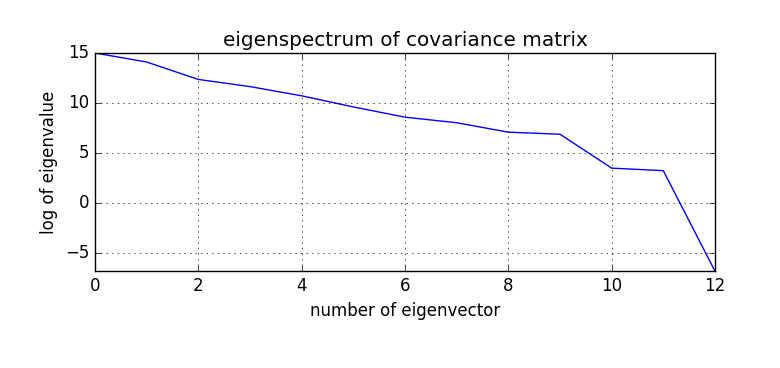
\includegraphics[width=16cm]{eig.png}
\caption{Eigenspectrum of the data}
\label{fig:eig}
\end{figure}

The PCA gave 13 principal components, of which only 2 were necessary to explain 90\% of the variance. This is verified by looking at the eigenspectrum plot in Figure \ref{fig:eig}. This plots the log of the eigenvalues against the principal component number. \\

\begin{figure}[h]
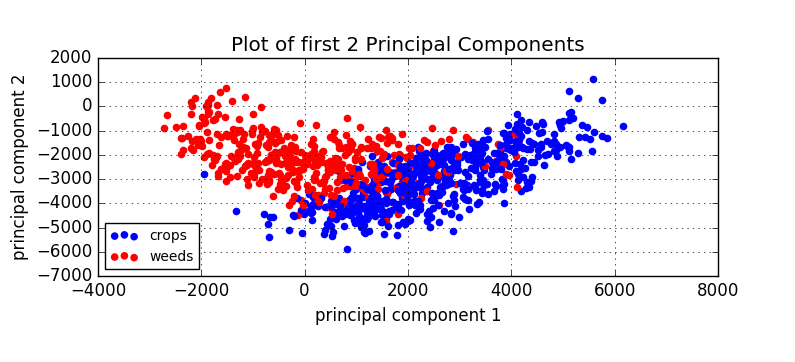
\includegraphics[width=16cm]{2pc.png}
\caption{Plot of the data projected onto the first two principal components}
\label{fig:2pc}
\end{figure}

The scatter plot in Figure \ref{fig:2pc} shows the data projected onto the first two principal components of the resulting 13. The legend can be used to identify the class of the points. \\

Looking at the plot, one can see how important these first 2 principal components are, as visually the clusters are mainly separated by their colours. In comparison, a plot of the data projected against the final 2 principal components is mostly concentrated around the center. \\

\subsection{Clustering}

The K-Means Algorithm was implemented using a combination of the\\ \texttt{sklearn.cluster.KMeans} package in Python, and previous code I had written for an assignment. The K-Means implementation was used with $k = 2$. The standard full K-Means algorithm was used with a maximum of 300 iterations. The cluster start points were initialised to the first 2 points in the training set.\\

\begin{figure}[h]
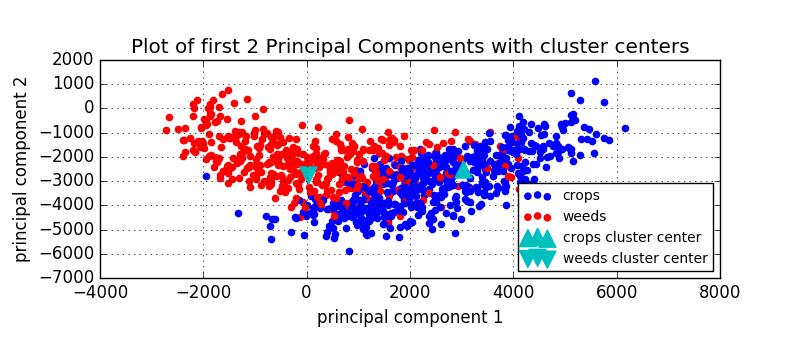
\includegraphics[width=16cm]{2pc_cc.png}
\caption{Plot of the data projected onto the first two principal components, with cluster centers from 2-Means clustering}
\label{fig:2pc_cc}
\end{figure}

The projection of the resulting cluster centers onto the first two principal components can be seen in Figure \ref{fig:2pc_cc}. From the plot, the K-Means algorithm performed very well on the data projected onto the first 2 principal components, as by-eye, each cluster center sits approximately in the center of each of the crops and weeds clusters. The algorithm classifies by measuring the distance between the test point and the two cluster centers, and returning the class of the closest cluster center. \\

The cluster centers were projected onto the first two principal components by taking the matrix of the cluster centers and performing the dot product of it against each principal component vector. This results in the projected clusters on each of the principal component vectors.

\newpage
\section{Generalization Bound for Learning with Multiple Feature Mappings}

\subsection{}

Note that a $\tilde{d}$-dimensional linear separator has $d_{VC} = \tilde{d} + 1$ \cite[p. 52]{abu}, where $\tilde{d}$ is the dimensionality of the transformed data $\in \mathcal{H}_Q$ by $\Phi_Q(\xbf)$.\\

In calculating the dimensionality of the new space, the different combinations of the original $(x_1...x_d)$ points to form the up to order Q monomials were considered. An upper bound may also be placed on the dimension of $\Phi_Q(\xbf)$ by the dimension of $\Phi_Q^+(\xbf)$, as this includes the repetition of identical terms, and therefore will be higher than $\Phi_Q(\xbf)$. To this end, if the terms are considered in order from Q = 0 up to Q, there are $d^Q$ combinations of each order monomial, such as:

\begin{equation*}
\begin{aligned}[c]
    Q=0, \\
    Q=1, \\
    Q=2, \\
    \\
\end{aligned}
\begin{aligned}[c]
    &1 \; &= d^0 = 1 \\
    &x_1, x_2, ..., x_d \; &= d^1 = d \\
    &x_1^2, x_1x_2, ..., x_d^2 \; &= d^2 \\
    \text{etc.}
\end{aligned}
\end{equation*}

Which results in $\tilde{d}$ equal to:

\[ \sum^Q_{i=0} d^i \]

and therefore $d_{VC}$ equal to:

\[ \big( \sum^Q_{i=0} d^i \big) + 1 \]

There are $(Q+1)$ terms in this sum, with the highest order polynomial equal to $d^Q$, which means that an upper bound can be placed on this, and:

\[ d_{VC} (\mathcal{H}_Q) \leq (Q + 1) \cdot d^Q  \]

\subsection{}
Using the bound in equation 2.14 \cite[p. 58]{abu}, and substituting in the value for the $d_{VC}$, to get the following bound, with probability at least $1 - \delta, \forall_{h \in \mathcal{H}_Q}$ (N.B. here, and from now on, I am using the derivations from the book, i.e. from the two-sided Hoeffding):

\[
    L(h) \leq \hat{L} (h, S) + \sqrt { \frac {8} {N} \ln \bigg( \frac {4 \cdot ( (2N)^{(Q + 1) \cdot d^Q} + 1) } {\delta} \bigg) }
\]

\subsection{}

If the polynomial kernel with the 2nd order transform is considered:

\[ \Phi_2(\xbf) = (1, x_1, x_2, ... x_d, x_d) \]

and then the product:

\[ \Phi_2(\xbf)^T \Phi_2(\xbf') = 1 + \sum^d_{i=1} x_ix_i' + \sum^d_{i=1} x_ix_jx_i'x_j' \]

which is equivalent to:

\[ 1 + (\xbf^T \xbf') + (\xbf^T \xbf')^2 \] \cite[p. 8-34]{abu} \\

For the Qth order transform, this product equals:

\[ \Phi_Q(\xbf)^T\Phi_Q(\xbf') = 1 + (\xbf^T \xbf') + (\xbf^T \xbf')^2 + ... (\xbf^T \xbf')^Q \\
= \sum_{i=0}^{Q} (\xbf^T \xbf')^i
\]

An upper bound on this can be placed as the Qth polynomial kernel, which equals:

\[ \sum_{i=0}^{Q} (\xbf^T \xbf')^i \leq (1 + \xbf^T \xbf)^Q \]

as it includes all the other terms from the sum, just with higher coefficients.\\

Note that I may bound $\Phi_Q(\xbf)$ by $\Phi^+_Q(\xbf)$, as it includes more terms due to the repeated identical terms, and if I set the repeated terms equal to 0, they are equivalent. \\

From the above, consider that:

\begin{align*}
    || \xbf || &\leq 1 \\
    \sqrt{ \langle \xbf, \xbf \rangle } &\leq 1 \\
    \langle \xbf, \xbf \rangle &\leq 1 \\
    \xbf^T \xbf &\leq 1 \\
    \xbf^T \xbf + 1 &\leq 2 \\
    (\xbf^T \xbf + 1)^Q &\leq 2^Q \\
    (\Phi_Q^+)T(\Phi_Q^+) \leq (\xbf^T \xbf + 1)^Q &\leq 2^Q \\
    \sqrt{\Phi_Q^+(\xbf)^T\Phi_Q^+(\xbf)} \leq \sqrt{ (\xbf^T \xbf + 1)^Q} &\leq \sqrt{2^Q} \\
    \sqrt{\langle \Phi_Q^+(\xbf), \Phi_Q^+(\xbf) \rangle} \leq \sqrt{ (\xbf^T \xbf + 1)^Q} &\leq \sqrt{2^Q} \\
    || \Phi_Q(\xbf) || \leq \sqrt{ (\xbf^T \xbf + 1)^Q} &\leq \sqrt{2^Q} \\
\end{align*}

\subsection{}

Consider that:

\[
|| \Phi_Q(\xbf) || \leq \sqrt{ 2^Q } \in \mathbb{R}^{\tilde{d}}
\]

from the above exercise.\\

Using an adjusted version of Theorem 3.8 \cite[p. 18]{mln}

\[ d_{VC} (\mathcal{H}_\rho) \leq \lceil \nicefrac{R^2} {\rho^2} \rceil \]

I adjusted this as I am considering the space of hyperplanes: $ \mathcal{H}_\rho = \{ (w) : || \wbf || \leq \nicefrac {1} {\rho} \}$. However, the input space is in $\mathbb{R}^{\tilde{d}}$ defined by $\Phi_Q (\xbf)$, so from the previous answer, as $\xbf$ is a ball of radius 1, in the tranformed space we have that $R = \sqrt{ 2^Q }$.\\

Plugging this into the above result yields:

\[ d_{VC} (\mathcal{H}_\rho) \leq \lceil \nicefrac { \big( \sqrt{ 2^Q } \big) ^2 } { \rho^2 } \rceil = \lceil \nicefrac{2^Q} {\rho^2} \rceil \]

Now, considering $\mathcal{H}$ as a nested sequence of subspaces, $\hh_1 \subset \hh_2 ... \subset \hh_d = \hh$, and defining $\hh_i = \hh_{\rho = \nicefrac {2^Q} {i}}$, where $i = \nicefrac {2^Q} {\rho^2}$. Also note that if $h = w \in \hh_i \setminus \hh_{i-1}$,
then $i = \lceil 2^Q \cdot || \wbf ||^2 \rceil $ as:

\begin{align*}
    || \wbf || \leq \frac {1} {\rho} \\
    || \wbf ||^2 \leq \frac {1} {\rho}^2 \\
    2^Q \cdot || \wbf ||^2 \leq \frac {2^Q} {\rho^2} \\
    \lceil 2^Q \cdot || \wbf ||^2 \rceil = i \\
\end{align*}

I can also take

\[
    \delta_i = \frac {1} {i}{i+1}
\]

Using the result from before gives:

\[ d_{VC} (\mathcal{H}_i) = i\]

which gives through Theorem 3.7 \cite[p.18]{mln}:

\[
    \mathbb{P} \Bigg\{
        \exists h \in \hh_i : L(h) \geq \hat{L} (h, S) +
        \sqrt {
            \frac {8} {n} \cdot \ln
            \frac  { \big(
            4 \big(
            ( 2n )^i + 1
            \big)
            \big ) } {\delta_i}
        }
    \Bigg\} \leq \delta_i
\]
 then, plug in and derive:
\[
    \mathbb{P} \Bigg\{
        \exists h \in \hh_i : L(h) \geq \hat{L} (h, S) +
        \sqrt {
            \frac {8} {n} \cdot \ln
            \frac { \big(
            4 \big(
                ( 2n )^\cw + 1
            \big)
            \cdot
            \big( \cw \cdot (\cw + 1) \big)
            \big) } {\delta}
        }
    \Bigg\}
\]
\[ =
    \mathbb{P} \Bigg\{
        \exists h \in \bigcup^d_{i=1 }\hh_i \setminus \hh_{i-1} : L(h) \geq \hat{L} (h, S) + \]
\[        \sqrt {
            \frac {8} {n} \cdot \ln
            \frac { \big(
            4 \big(
                ( 2n )^\cw + 1
            \big)
            \cdot
            \big( \cw \cdot (\cw + 1) \big)
            \big) } {\delta}
        }
    \Bigg\}
\]
\[ = \sum^d_{i=1}
    \mathbb{P} \Bigg\{
        \exists h \in \bigcup^d_{i=1 }\hh_i \setminus \hh_{i-1} : L(h) \geq \hat{L} (h, S) + \]
\[        \sqrt {
            \frac {8} {n} \cdot \ln
            \frac { \big(
            4 \big(
                ( 2n )^\cw + 1
            \big)
            \cdot
            \big( \cw \cdot (\cw + 1) \big)
            \big) } {\delta}
        }
    \Bigg\}
\]
\[ = \sum^d_{i=1}
    \mathbb{P} \Bigg\{
        \exists h \in \hh_i \setminus \hh_{i-1} : L(h) \geq \hat{L} (h, S) + \]
\[        \sqrt {
            \frac {8} {n} \cdot \ln
            \frac { \big(
            4 \big(
                ( 2n )^\cw + 1
            \big)
            \cdot
            \big( \cw \cdot (\cw + 1) \big)
            \big) } {\delta}
        }
    \Bigg\}
\]
\[ = \sum^d_{i=1}
    \mathbb{P} \Bigg\{
        \exists h \in \hh_i \setminus \hh_{i-1} : L(h) \geq \hat{L} (h, S) +
        \sqrt {
            \frac {8} {n} \cdot \ln
            \frac { \big(
            4 \big(
                ( 2n )^i + 1
            \big)
            \cdot
            \big( i \cdot (i + 1) \big)
            \big) } {\delta}
        }
    \Bigg\}
\]
\[ \leq \sum^d_{i=1}
    \mathbb{P} \Bigg\{
        \exists h \in \hh_i : L(h) \geq \hat{L} (h, S) +
        \sqrt {
            \frac {8} {n} \cdot \ln
            \frac { \big(
            4 \big(
                ( 2n )^i + 1
            \big)
            \cdot
            \big( i \cdot (i + 1) \big)
            \big) } {\delta}
        }
    \Bigg\}
\]
Then using Hoeffding's
\[
    \leq \sum^d_{i=1} \delta_i = \sum^d_{i=1} \frac {1} {i \cdot (i + 1)} =
    \delta \sum^d_{i=1} \frac {1}
    {i \cdot (i + 1)} \leq \delta \sum^\infty_{i=1} \frac {1} {i \cdot (i + 1)} = \delta
\]

This model of proof was taken from the lecture notes. \cite[p. 19]{mln} \\

Therefore, the bound on $h$, w.p. at least $ 1 - \delta$ is:

\[
    L(h) \leq \hat{L} (h, S) +
    \sqrt {
        \frac {8} {n} \cdot \ln
        \frac { \big(
        4 \big(
            ( 2n )^\cw + 1
        \big)
        \cdot
        \big( \cw \cdot (\cw + 1) \big)
        \big) } {\delta}
    }
\]


\subsection{}

% For each hypothesis space $\mathcal{H}_1, \mathcal{H}_2 ..., \mathcal{H}_Q$, note that:
%
% \[
%     $\mathcal{H}_1 \subset \mathcal{H}_2 \subset ... \subset \mathcal{H}_Q$
% \]
%
% as each polynomial transform that describes the hypothesis space includes the monomials of order i $in \mathcal{H}_i$, and adds the monomials of order Q.
%
% From this, the union of the sets

The VC dimension is defined as the largest N such that $m_\mathcal{H} (N) = 2^N.$
It is also true that $m_\mathcal{H} \leq \min \; (|\mathcal{H}|, 2^N)$
\cite[Home Assignment 5.2.1]{mla}. Finally, if $m_\mathcal{H} (N) = 2^N \; \forall_N, d_{VC} = \infty$. \cite[def. 2.5, p.50]{abu}\\

As $|\mathcal{H}|$ is infinite for the union of all polynomial transformations, for all N, $m_\mathcal{H} = 2^N$, and following the definition above, this implies that $d_{VC} = \infty$.

\subsection{}

\newpage
\printbibliography
\end{document}
